
         \begin{figure}[h]
            \centering
            \begin{tikzpicture}
               %图片
               \node at (0,0) {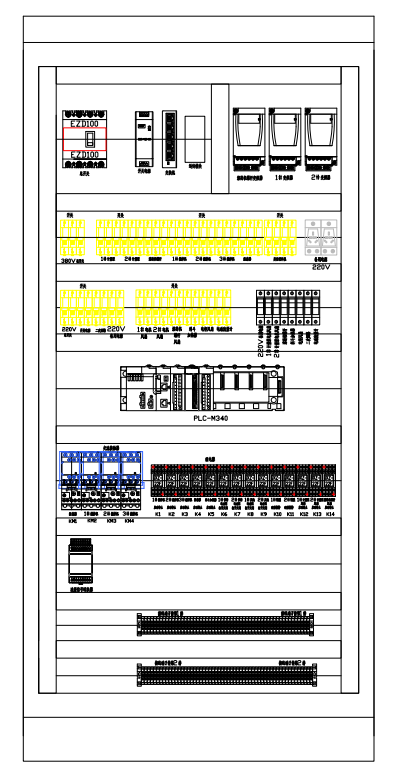
\includegraphics[height=10cm]{g04.PNG}};

               %说明
               \def \itemNumber {1};
               \def \centertPoint {-1.9, 2.7};
               \node at (-3,3) (\itemNumber) [text_box] {电柜总开关};
               \draw (\centertPoint) rectangle +(0.8,0.9)[red];
               \def \itemNumber {2};
               \def \centertPoint {-1.9, 1.5};
               \node at (-3,2) (\itemNumber) [text_box] {其余开关};
               \draw (\centertPoint) rectangle +(3.2,0.7)[red];
               \def \itemNumber {3};
               \def \centertPoint {-1.9, 0.6};
               \node at (-3,1) (\itemNumber) [text_box] {其余开关};
               \draw (\centertPoint) rectangle +(2.4,0.7)[red];

            % 辅助线
               \def \xLimit {8};
               \def \yLimit {7};
            %    
			% 辅助线
            \draw (-\xLimit,-\yLimit) [help lines] grid (\xLimit,\yLimit);
            \foreach \x in {-\xLimit, ...,\xLimit}{
               \node [red] at (\x, \yLimit) {\x};
               \node [red] at (\x, -\yLimit) {\x};
               \node [red] at (\x, 0) {\x};
            }
            \foreach \y in {-\yLimit, ...,\yLimit}
                  \node [red] at (-\xLimit, \y) {\y};
            \foreach \y in {-\yLimit, ...,\yLimit}
                  \node [red] at (\xLimit, \y) {\y};
            \foreach \y in {-\yLimit, ...,\yLimit}
                  \node [red] at (0, \y) {\y};


            \end{tikzpicture}
            \caption{电柜内布局}\label{fig:p6}
         \end{figure}

